\chapter{Using the Choreographer}\label{sec:usingthe}

This section is a short user manual for the Choreographer project.
Step by step, the actions to be undertaken in order to create and execute a choreography are detailed.\\

In this chapter it is assumed that the following are available:
\begin{itemize}
\item A computer running the Windows ( 7 or above ) operating system.
\item A functional wireless serial port device connected.
\item One or more Cubli robots with the choreography firmware flashed.
\end{itemize}

\section{Preparation: Testing and Training Cubli}

This is an \textit{optional} step, which consists in:

\begin{itemize}
\item[] Turning Cubli on, and checking that the batteries are full
\item[] Through the mode button, having Cubli perform all the basic moves on the proper surface until it has mastered them.
\end{itemize}

Taking these precautions results in smoother choreographies, and ensures that the Cubli robot is functional.

\section{Connecting to Cubli}

First, launch the choreographer app, available as an executable in the github repository.

Once the app is launched, a serial port selection and settings dialog pops up ( \textit{c.f. Figure \ref{img:SerialSettings}} ). Select the appropriate serial port. It must correspond to a wireless serial device connected to the pc.

\begin{figure}[ht]
   \centering
   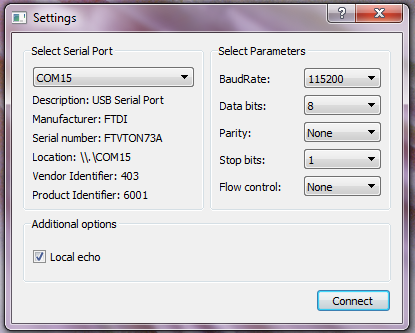
\includegraphics[width=0.75\textwidth]{img/SerialSettings.png}
   \caption{Settings Window for the serial port, displaying an example of correct values.}
   \label{img:SerialSettings}
\end{figure}

\textbf{Note:} If closed, the settings dialog remains available through the menu bar of the main window.\\

At this point, turning on a Cubli will automatically connect it to the application and its timeline should appear. You can also manually attempt to connect to Cublis which are powered on, by pressing the large '+' button in the middle of the main window.


\section{Make Your Own Choreography}

Once a cube's timeline is visible, it is possible to create or modify the choreography by using the mouse buttons within its bounds - that is, the white area.\\

On an empty part of the timeline, left-click once to create a primitive.

Left-click that primitive again to change its type.

Click-and-drag the primitive to modify the timing.

Right-click any primitive to delete it.\\

Information concerning the last-clicked primitive is visible in the top panel of the main window.\\

\textbf{Note:} when moving a primitive, it follows your mouse unless there isn't any space for it.\\

When cycling through primitive types, due to the change of length, it is possible that a primitive no longer fits between the ones surrounding it. In this case all the following primitives are displaced to make space.\\

Interact with the various timelines until you are satisfied with the choreography.


\section{Sync Your Choreography to the Cubes}

Press the apply button and wait for the app status to show "Sync Successful".\\

\textbf{Note:} It sometimes occurs that a cube does not respond too long while syncing, in which case the sync is cancelled by the application, and that cube is disconnected. In that case, ensure that the cube is turned on and functional before trying again.\\

Once the sync is successful, all connected cubes have the choreography stored in the exact state it was when the apply button was pressed. 
At this point further modifications to the timelines in the app will not be synced until the apply button is pressed again.\\

\textbf{Note:} Timelines are not deleted from the editor panel when a cube is disconnected, in order to prevent accidentally deleting choreography data. As such, they remain visible, but will not be synced until the cube is reconnected. Reconnecting to a cube is the same process as in the '\textit{Connecting to Cubli}' step above.\\

\textbf{Note:} In addition, when Cubli is turned off, all timeline information is cleared from its memory. As a result, it is necessary to once again sync any cube that has been restarted.




\section{Run the Choreography}

Once a timeline is stored in the cube, it is ready to execute the choreography. 

In order to do so press the "Play" button.\\

This will initiate a countdown to the start of the choreography, during which all cubes must confirm that they are performing. If one cube or more do not provide confirmation the choreography is cancelled and must be attempted again. The non-responsive cube is automatically marked as disconnected.\\

It is also possible to manually cancel the countdown by pressing the "Play" button, which is at this point displaying the countdown value.\\

After the countdown the choreography is started, and cubes will attempt to complete their current primitive even if they fail. No user interaction with the app is necessary, however in the event that they fall on an unrecoverable face, Cublis must manually be reset back to their main face.

\begin{figure}[ht]
   \centering
   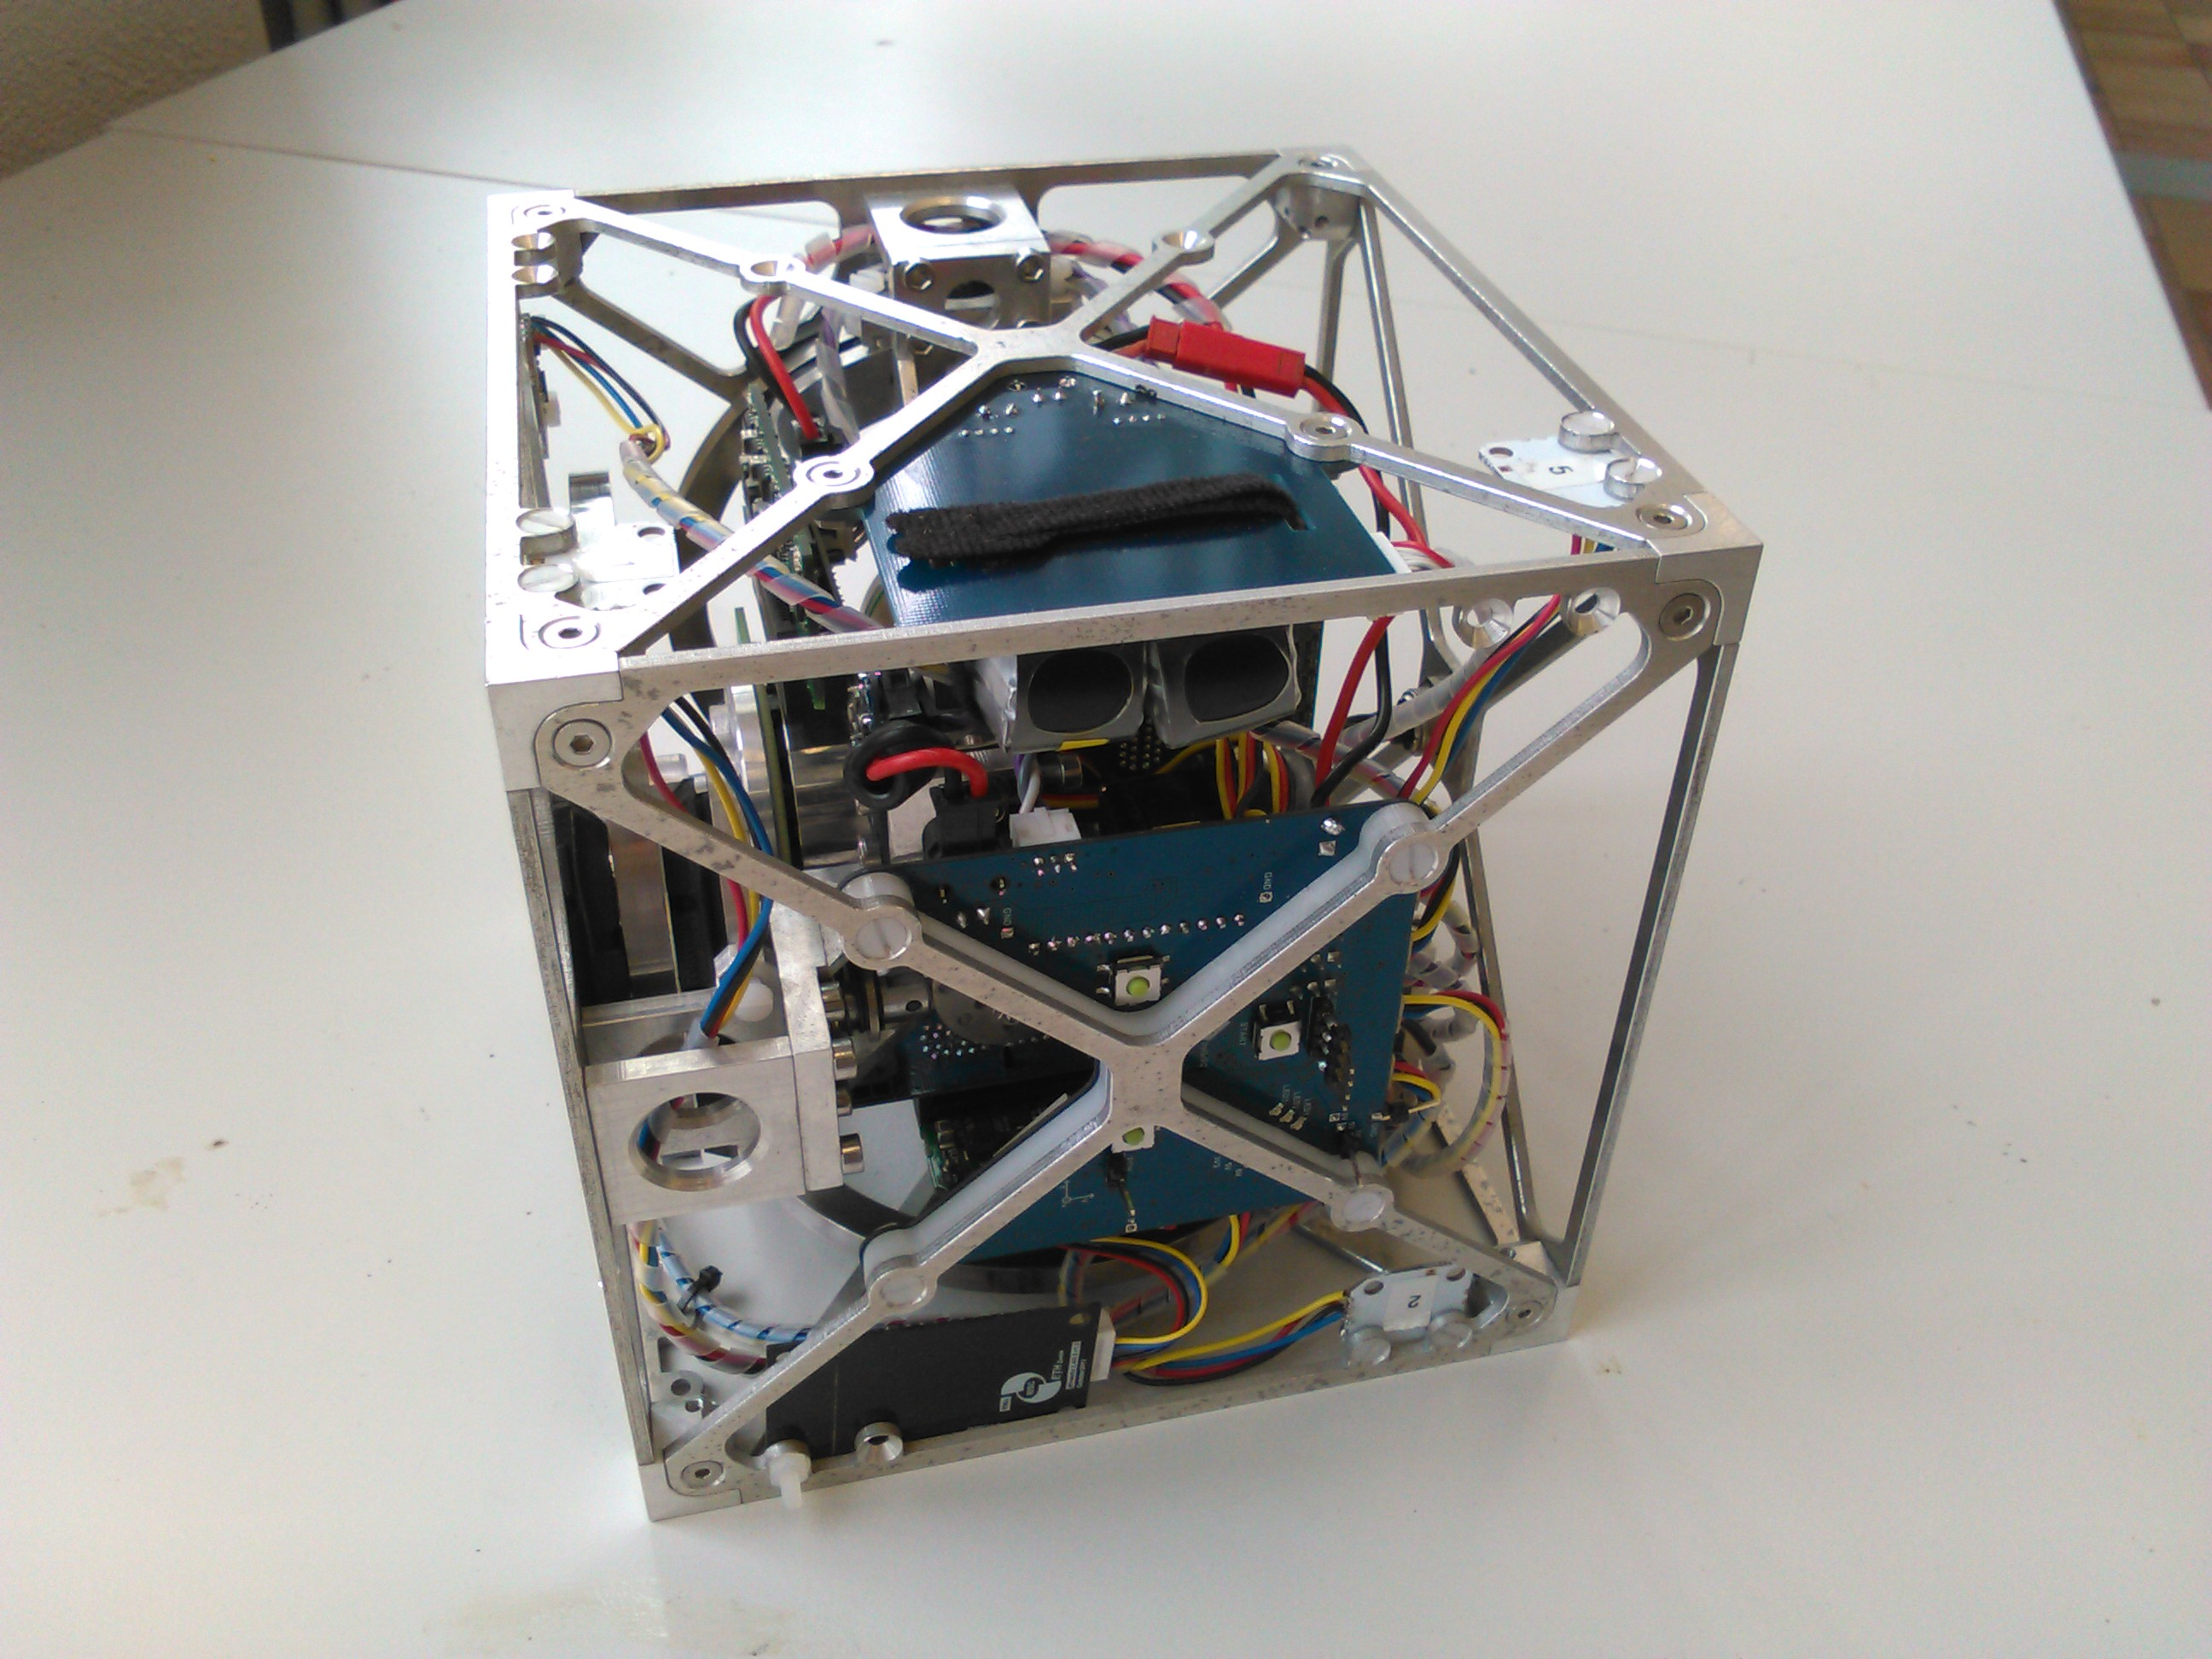
\includegraphics[width=0.75\textwidth]{img/MainFace.jpg}
   \caption{Cubli set-up on its main face. Note the orientation of the buttons on the front-facing panel.}
   \label{img:MainFace}
\end{figure}


\section{Stop the Choreography}

The choreography stops automatically when it reaches its natural end, that is when all cubes have completed their last primitive. \\

It is also possible to stop it manually, by pressing the "Stop" button, which can be seen in place of the "Play" button in the UI once the choreography is running.